%%%%%%%%%%%%%%%%%%%% author.tex %%%%%%%%%%%%%%%%%%%%%%%%%%%%%%%%%%%
%
% sample root file for your "contribution" to a contributed volume
%
% Use this file as a template for your own input.
%
%%%%%%%%%%%%%%%% Springer %%%%%%%%%%%%%%%%%%%%%%%%%%%%%%%%%%


% RECOMMENDED %%%%%%%%%%%%%%%%%%%%%%%%%%%%%%%%%%%%%%%%%%%%%%%%%%%
\documentclass[graybox]{svmult}

\usepackage{mathptmx}       % selects Times Roman as basic font
\usepackage{helvet}         % selects Helvetica as sans-serif font
\usepackage{courier}        % selects Courier as typewriter font
\usepackage{type1cm}        % activate if the above 3 fonts are
                            % not available on your system
%
\usepackage{makeidx}         % allows index generation
\usepackage{graphicx}        % standard LaTeX graphics tool
                             % when including figure files
\usepackage{multicol}        % used for the two-column index
\usepackage[bottom]{footmisc}% places footnotes at page bottom

% see the list of further useful packages
% in the Reference Guide

\makeindex             % used for the subject index
                       % please use the 

%%%%%%%%%%%%%%%%%%%%%%%%%%%%%%%%%%%%%%%%%%%%%%%%%%%%%%%%%%%%%%%%%%%%%%%%%%%%%%%%%%%%%%%%%

\begin{document}

\title*{Metagenomic design and sequencing}
% Use \titlerunning{Short Title} for an abbreviated version of
% your contribution title if the original one is too long
\author{William L. Trimble, Stephanie M. Greenwald, Sarah Owens, anyone else who wants a piece }
% Use \authorrunning{Short Title} for an abbreviated version of
\authorrunning{Trimble, Greenwald, and Owens}
% your contribution title if the original one is too long
\institute{William L. Trimble, Stephanie M. Greenwald, and Sarah Owens  \at Institute for Genomics and Systems Biology, University of Chicago \email{name@email.address} } 
%   \and Name of Second Author \at Name, Address of Institute \email{name@email.address}}
%
%
\maketitle

% "starred" for online
\abstract*{
Abstract summarizes the paper in a 10--15 lines for indexing, discovery, and marketing}

% Use the plain \texttt{abstract} command if the abstract is also to appear in the printed version of the book.}
\abstract{Abstract summarizes the paper in a 10--15 lines for indexing, discovery, and marketing (for print) } 

\section{The technology}
\label{sec:1}

The technological advances in sequencing technology in the recent decade have made determining the sequence nucleic acid polymers affordable and widespread.  While the study of variations in the genomes of model organisms including humans is a rich and fruitful area of investigation, microorganisms have vastly greater numbers and sequence diversity than macroorganisms.  Sequencing of DNA from environmental samples has become a fast-growing application of sequencing technology.

Metagenomics is the analysis of genetic material extracted from environmental samples or extracted from mixtures of organisms.  Two general approaches are available, targeted gene sequencing and random "shotgun" sequencing.    Targeted sequencing amplifies gene fragments of interest using PCR primers corresponding to conserved regions of selected genes.   Subsets of the sequence of the prokaryotic  rRNA 16S subunit, the internal transcribed spacer (ITS) in fungi, functional genes of interest to oxidation-reduction metabolism(NifH, AmoA), and conserved non-RNA phylogenetic marker genes (XXX) are all suitable.  The 16S rRNA gene has proven most popular for surveying the composition of microbial communities, and as one of the genes that has been under investigation for the longest, its primers and sequences have been the most studied and have the largest number of database sequences.

Random, called "shotgun" sequencing provides unaligned samples from each organism's thousands of genes, rather than amplifying a single gene per organism or organismal type.  This increases the complexity of the sequencing product several thousandfold, and as a result, much greater per-sample sequencing effort is required.
This higher sequencing effort has meant that environmental shotgun sequencing has been enabled disproportionately by low-cost sequencing technologies, and as a consequence the total amount of shotgun sequence data has XXX HISTORICALGRAPH.
Gigabase to few-tens-of-gigabase samples have been fashionable and common.  Sequencing single samples to depths of a hundred gigabases or greater have been uncommon but not unheard of.

Generally, researchers are interested in the effect of external variables on the composition of microbial communities.  For both the targeted-gene and shotgun approaches, a vector of inferred relative taxonomic abundances is produced.  For shotgun sequencing, the sequences can be further interpreted as relative abundances of fragments from different functional classes of genes.  Analytical approaches that use additional information (from comparative genomics, or from chemical reaction networks) to extend the inferred profiles are in current use.  (XXX examples, PRMT, HUMANN's operon-exploit)

Finally, we can confidently recommend engaging the specialists in the wetlab and in computational analysis early in the sequencing process.  
\section{Experimental design guidelines}
\label{sec:2}
% Always give a unique label
% and use \ref{<label>} for cross-references
% and \cite{<label>} for bibliographic references

The general aspects of experimental design for metagenomics are similar to those for RNA-seq experiments.  

, where the relationship between dynamic range and sample number is the principal design constraint. (Auer)    While there is evidence of diminishing returns on RNA-seq sampling in excess of 10 million tags (2 gigabases with 2x100 cycle sequencing reads) for eukaryotic RNA-seq (Wang), shotgun metagenomic samples typically target 10 gigabases per sample.     This allows 1 or 2 samples per Miseq flowcell  (7 million spots at 400~bp per spot) and as many as 4 samples per Hiseq flowcell at 2x101.

Read-length requirements differ from RNA-seq experiments, however.   While RNA-seq experiments can quantify expression with short (30- or 50-bp) sequence tags,  individual RNA-seq reads need only reliably inform the position(s) in the reference sequence they represent.   Individual metagenomic reads must identify which organism they come from and what (which biochemical entity) they represent for exploitation, and the reads must do so individually, since each random fragment may or may not be from the same organism.  This makes longer reads--reads in the range of 150-450~bp--more valuable for exploitation than even overwhelming numbers of short reads.   On the other side of the read-length continuum, the anonymous nature of individual reads makes sequencing technologies that produce very long reads with very poor (10\%) sequencing error rates (Pacific Biosciences, Oxford Nanopore) choices for metagenomics unless complemented with data with high base accuracy.  The simultaneous detection of the likely organism and the likely corrected sequence is not currently feasible with only long-read low-quality data except perhaps in the lowest complexity samples.

The innovation of synthetic sample-labeling oligomers known as barcodes allows multiple samples to be sequenced simultaneously in the same flowcell at the same time.  This ability is principally thought of as a way to increase the number of samples per instrument run, but has applications in balancing sequencing effort.    Auer and ..   have suggested using barcodes to construct blocked experimental designs that control, for instance, per-lane technical effects.   It has been our experience that the technical repeatability within platforms is very good, but batch effects between different types of sequencing (different read lengths, ABISolid vs. 454 vs. Illumina) and different types of library preparation (use of different PCR parameters for different samples, use of Multiple Displacement Amplification) persist.  Block designs to test for or balance technical variation are better spent on the factors of the experiment,  XXX

Biological samples are much more valuable than technical samples in supporting the detection of significant differences between treatments).  Since pooling of samples can be done in-silico, but samples cannot be un-pooled, pooling precludes estimation of variation within the treatment groups, and is not recommended.

The large complexity difference between shotgun and targeted gene surveys and the availability of protocols to multiplex more than 600 samples in a single sequencing run invite researchers to sequence large numbers of samples with just a single gene, and to apply shotgun sequencing to selected samples.   Another sequencing option is to one or a small number of samples to much greater sequencing depth than the others.  This approach is not recommended, as it (by definition) consumes large amounts of sequencing effort that would usually be better applied to more samples to permit characterization of the within-group variability of sequence signals.

\subsection{Platform differences}

\begin{table}
\caption{Sequencing platforms suitable for metagenomic sequencing.}
\begin{tabular}{rrrrrrrrrrr}
Platform
454  & 150 & 200 & 300 & 400 & 500 & 800 & 1000 & 1500  \\
Illumina Miseq & 10\% & 10\% & 10\% & 10\% & 5\% & 5\% & 5\% & 2\%  \\
Illumina Hiseq & 5 & 5 & 4 & 4 & 3 & 3 & 3 & 4  \\
IonTorrent & 200 & 200 & 200 & 200 & 200 & 200 & 200 & 200  \\
ABIsolid & 430 & 180 & 80 & 55 & 80 & 50 & 40 & 15  \\
PacBio & 430 & 180 & 80 & 55 & 80 & 50 & 40 & 15  \\
Oxford Nanopore  & 430 & 180 & 80 & 55 & 80 & 50 & 40 & 15  \\
\end{tabular}
\end{table}

Because of the high complexity of metagenomic samples, individual reads contribute little to the genetic characterization of the entire sample, and require recognition of some kind before they are invested with meaning.

ABIsolid has been applied to metagenomics, but the short read lengths (ca. 50 bp) present a challenge both to assembly and short-read annotation.
Iontorrent has been applied successfully to targeted-gene metagenomic analysis; barcodes permitting as many as X samples at XXX depths are commercially available.  Shotgun metagenomics with Iontorrent is somewhat more risky because error correction for assembly is much more computationally expensive than error correction for targeted gene analysis.  There some new approaches that are lowering the computational burden of error correction and assembly on very complex datasets, particularly probabilistic data structures.


\subsection{Sample replicates} 
\label{subsec:2}


Auer and XXX suggest block designs to control for lane effects, and additional controls for barcode effects can be imagined.  Modern sequencers have batch effects that can bias end results, but these seem to be related to the overall protocol, including fragmentation methods and PCR conditions, not to specific lanes simultaneously sequenced on an instrument.    An instrument has a chance of having some of the output fail to produce usable or high-quality output; a single lane can fail, or fail to produce high sequence quality or quantity, at the same time that adjacent lanes produce good sequence.
The principal benefit of a design that spreads samples across several lanes is that this design provides  insurance against a technical failure that is confined to a single lane.  If one lane fails, a loss of one eighth of the sequencing depth is less disruptive to experimental design that the loss of data for one eighth of the samples.   Block randomization is clearly indicated, however, if the sequencing protocol, whether extraction, template construction or purification, or sequencing chemistry or platform changes.

Sometimes* some sequencing samples fail.   Despite the best efforts, some samples fail to cluster, and some sequencing runs suffer problems that result in unusable sequence data.  It is essential to plan for the possibility
* More often than anyone wants

\subsection{Sample requirements }
\label{subsec:4}
%
When creating metagenomic sequencing libraries the quality and quantity of the genetic material to be sequence is of great importance. The quantity of material varies from method to method and can be anywhere from 1~ng – 1ug of material. It is important to make sure that the amount of genetic material available for library preparation falls within the range given by the kits protocol.
%
More important is the quality of the nucleic acids. Even if a researcher has ample genetic material, if the material is not of good quality a robust library often cannot be made. Good quality starts from sample collection and will be affected by the samples environment. For instance, samples taken from hot or acid rich environments will be innately lower in quality compared to a sample taken from a relatively cold or more neutral environment.
%
The proper storage of a sample also plays a huge role in overall sample quality. We recommend storing samples at -80°C as soon as possible after collection and avoiding free-thaw cycles. Steps used to maintain high quality through the extraction process are detailed below.
%
The composition of the microbial communities in environmental samples can shift depending on the conditions of sample storage. Storage variables such as duration of time and temperature can drastically affect the abundance of different members in the communities and create biases. Bray-Curtis analysis can be used to determine how these communities shift (Rubin et al., 2013). We recommend that extraction of the genetic material happen as soon as possible after sample collection to reduce storage associated community shifts. Alternately, immediately freezing samples at    -80°C after collection can reduce community shifts
%
To assess the quantity of a sample after extraction we recommend Invitrogen’s Qubit Fluorometer. The qubit determines the starting concentrations of given samples by utilizing a fluorescent dye that binds to nucleic acids for quantification. We recommend avoiding the Nanodrop, as it consistently overestimates nucleic acid concentrations. Unlike the Nanodrop, the Qubit Fluorometer can discriminate between DNA and contaminants, such as RNA.
%
To assess the quality of the genetic material we recommend using Agilent’s 2100 Bioanalyzer or an agrose gel to view the genetic material. Generally, high quality genetic material destined for metagenomic research will be free of any fragments below 100-200~bp.  If the number of fragments 200~bp out-number the rest this is an indication of fragmentation and this low quality genetic material.

\section{Wetlab protocol}
There are two main metagenomic library types/kits that have been tested thoroughly and are confidently recommend for metagenomic sequencing.  These two types are the TruSeq and the Nextera, both from Illumina, Inc.(San Diego, California). These two library types differ in their approach in two key components of metagenomic library generation: the fragmenting or shearing of the input material and the ligation of sequencing adaptors and identifying barcodes. 
Multiple factors may impact the selection of a kit for metagenomic library generation such as: desired insert size, amount of input DNA available, and the availability of a mechanical shearing device (sonicator).
Detailed below are protocols that address the creation of Nextera and TruSeq metagenomic libraries. 

Materials
\paragraph{Kits, Reagents, and Consumables}
\begin{enumerate}
\item{    Qubit HS Assay, for Invitrogen’s Qubit Fluorometer}
\item{       Agencourt Ampure XP Beads}
\item{       microTube AFA Fiber Pre-Slit with Snap-Cap 6X16mm, for Covaris S-series}
\item{       Illumina’s TruSeq PCR-free Sample Prep*}
\item{       Illumina’s Nano DNA Sample Prep Kits*}
\item{       Kapa Biosystems Library Amplification kits*}
\item{       Wafergen’s PrepX Complete ILMN DNA library Kits}
\item{       Absolute Ethanol}
\item{      Agarose (select agarose according to DNA fragment size)*}
\item{      Life Technologies’s E-Gels (1.5\%)*}
\item{      Blue Pippin Prep DNA Gel Cassettes 3\%, 2\%, 1.5\%, or 0.75\%}
\item{    Bio-O Scientific’s Nextflex DNA Barcodes and PCR mixture}
\item{      Illumina’s Nextera DNA kit}
\item{      ZymoTM Purification Kit (ZR-96 DNA clean and ConcentratorTM-5)}
\item{    Agilent DNA HS kit}
\item{      MoBio PowerSoil DNA isolation Kit}
\item{      Smart Spatula}
\end{enumerate}
* Indicates an alternative protocol/kit to the recommended one

\paragraph{Equipment}
\begin{enumerate}
\item{    Invitrogen’s Qubit Fluorometer}
\item{      Covaris S-series system}
\item{      Wafergen’s Apollo 324 system}
\item{      Magnetic Stand or Rack (holds 1.5ml or 96 well plates)}
\item{      Thermocycler}
\item{      Sage Science’s Blue Pippin Prep}
\item{      Agilent 2100 Bioanalyer}
\end{enumerate}

\subsection{Library Types}
For the generation of metagenomic libraries, we recommend two main types: TruSeq libraries and Nextera libraries.  TruSeq libraries have been on the market longer, so there are more kits and biotechnology companies that cater to their creation. 
Nextera libraries are newer and, to date can only be made with Illumina reagent kits.  
The main different between Nextera libraries and TruSeq libraries is the fragmentation procedure. 
To generate any metagenomic library the DNA much be sheared to create blunt ends that sequencing adaptors can ligate to. TruSeq library generation relies on mechanical sonication to fragment DNA. Nextera library generation uses an engineered enzyme to simultaneously fragment and tag input material. Based on these differences. Further, when creating a TruSeq library as compared to a Nextera library, the user has greater control over the insert size of library fragments.  Increased control of insert size can be especially useful with certain bioinformatics platforms. TruSeq and Nextera library preparation also varies in regards to the amount of input material needed. TruSeq library generation generally requires 500-1,000~ng of input material, while Nextera needs only 50~ng. Generation of Nextera libraries is particularly helpful with low biomass samples.

\subsection{Positive and negative controls }

There are numerous controls utilized throughout metagenomic library preparation in order to ensure unbiased and good quality data. The first of these controls is the extraction blank, a negative control. When extracting DNA for the metagenome researchers will include 1-3 extraction blanks with the sample set. The researcher will then compare the quality and quantity of the extraction blank to the samples and if a sample is found to match the extraction blank it will be discarded as a false positive.
%
The second of these controls is the library blank and is used in the same manner as the extraction blank. Water will be run through the library preparation process in tandem with the samples and used to remove false positives from the set.
%
Use of a negative control during library preparation is more common during the PCR step and several negative controls will often be included. This is because primer-dimers will often be generated by PCR along with the amplified libraries. Researchers will use the nucleic acid concentration of the negative controls to determined the concentration of primer-dimers in any given sample, often called the background noise.
%
Researchers also employ positive controls in metagenomic preparation. These positive controls consist of sequences of DNA that are of high quality, well studied, and explicitly known. The most common positive control is called PhiX. These positive controls can either be spiked into the samples as an internal control or they can be run by themselves as an external control. The positive controls are then compared to the individual samples to help determine the quality of the library and the effectiveness of the library preparation method.

DNA Extraction
[MoBio PowerSoil DNA isolation Kit]

\subsection{DNA Quantification}

It is recommended to start with 500~ng of high-quality DNA for TruSeq metagenomic library prep, although lower quality and concentrations may be used. However, this may lead to lower quality sequencing data and more observed sequencing bias. If a Nextera metagenomic library is being prepared the protocol is optimized for exactly 50~ng.

We recommend the following protocol:
\begin{enumerate}
\item{     Make a Qubit working solution by diluting the Qubit DNA reagent 1:200 in Qubit DNA buffer using a sterile plastic tube.}
\item{       Load 190~ul of Qubit working solution into tubes labeled standard 1 and 2.}
\item{       Add 10~ul of standard 1 solution and standard 2 solution to the appropriate tube and mix by vortexing for 2-3 seconds.}
\item{         Note: These are positive and negative controls used to calibrate the instrument.}
\item{       Load 198~ul of Qubit working solution into each individual assay tube.}
\item{       Add 2~ul of DNA to each assay tube and mix by vortexing 2-3 seconds. The final volume of this solution should equal 200~ul.}
\item{        Note: The amount of sample and working solution added to each assay tube can vary depending on concentration of the sample. The sample can vary between 1-20~ul, and the working solution can vary between 199-180~ul with the final volume equaling 200~ul. It is recommended to use 2~ul of sample to produce the most accurate results.}
\item{       Allow all the tubes to incubate at room temperature for 2 minutes.}
\item{       Select DNA assay on the Qubit Fluorometer. Select run a new calibration.}
\item{       Insert the tube containing Standard 1, close lid and press read.}
\item{       Remove standard 1 and repeat step 8 for standard 2.}
\item{      Insert sample, close lid and press read.}
\item{      Calculate concentration using dilution calculation on Qubit Fluorometer by selecting original volume of sample added to the assay tube.}
\item{      Repeat step 10 and 11 until all samples have been quantified.}
\end{enumerate}

\subsection{TruSeq Metagenomic Library Prep}
\subsubsection{ Insert Size Determination}

Insert size determination is an important consideration for TruSeq library prep. Due to the enzymatic shearing of Nextera libraries, the ratio of DNA to enzyme and the enzymatic cut sites will determine the insert size of a Nextera library. For TruSeq library prep, however, it is critically important to determine what library insert size will work best for your downstream analysis. Often, bioinformaticians will have a preference. We recommend consulting with any bioinformaticians that will be analyzing data before making your libraries. We also recommend the following guidelines seen in Figure 1. A 170-180 base pair insert (270-280~bp including adaptors) will result in overlapping reads on a 2X100~bp Hiseq run. A 250 base pair insert  (350~bp with adaptors) will result in over lapping reads on a 2X150 Hiseq run. A 500 base pair insert (600~bp with adaptors) will result in no overlap on a 2X100 or 2X150 Hiseq run. Finally, a 300-400 base pair insert (400-500~bp with adaptors) will result in no overlap with a known distance between the reads for single genome assembly.

\subsubsection{Shearing of Libraries}

For TruSeq libraries we recommend using the Covaris S-series system for mechanical shearing. The following instructions pertain to the S2 system but can be easily adapted to the S1 series through consulting the manual.  We recommend setting the water bath between 6-8°C and using a minimum of 500~ng sample in 50~ul-100~ul. It is important to use no less then 50~ul of sample as the Covaris relies on surface area to appropriately shear the material. If there is not at least 500~ng in 100~ul, we recommend using Agencourt Ampure XP Beads to concentrate the sample down to a smaller volume using a 1.8X bead ratio.  The conditions set on the Covaris are directly related to the preferred insert size of the final library, use the following table to determine what conditions to use for shearing.

\begin{table}
\caption{The input protocols for a S2 Covaris to achieve a peak at a given base pair length.}
\begin{tabular}{rrrrrrrrrrr}
Target Base Pair (Peak) & 150 & 200 & 300 & 400 & 500 & 800 & 1000 & 1500  \\
Duty Cycle & 10\% & 10\% & 10\% & 10\% & 5\% & 5\% & 5\% & 2\%  \\
Intensity & 5 & 5 & 4 & 4 & 3 & 3 & 3 & 4  \\
Cycles per Burst & 200 & 200 & 200 & 200 & 200 & 200 & 200 & 200  \\
Time (Seconds) & 430 & 180 & 80 & 55 & 80 & 50 & 40 & 15  \\
\end{tabular}
\end{table}

We recommend the following protocol:
\begin{enumerate}
\item{      After determining an appropriate insert size for the libraries use Table 1 to program the Covaris with the size specific operating conditions.}
\item{      Bring the water bath to 6-8°C while letting the Covaris de-gas for at least 30 minutes}
\item{      Aliquot 500~ng of each sample in 50~ul-100~ul into separate Covaris microTubes.}
\item{      Insert each Tube into the Covaris adaptor on the head of the instrument, submerge the head of the instrument into the water-bath.}
\item{      Hit the start button on the control software in order to initiate the given operating conditions, and let the program run its duration.}
\item{      Take out the microTube and set it aside on ice}
\item{      Repeat steps 4-5 for all samples}
\end{enumerate}

\subsubsection{Choosing adaptors and multiplexing}

We recommend using Illumina standard indexes (Table 2) when generating TruSeq libraries. When multiplexing, it is important to choose barcodes for individual samples that will be complementary to the barcodes of other samples in the same pool/sequencing lane. During sequencing, bases A and C are found in the red channel and bases T and G are found in the green channel. To ensure data quality, it is essential that the sequencer be able to detect a good proportion of bases in each channel. During the index read, this can be particularly challenging, as there are fewer bases present (just the indexes instead of the biologically expected 25\% of each base). For example, if a pool only contained samples with index 1 and 2, during the first read of the index the machine would only detect samples in the red channel (base A for index 1 and base C for index 2) and the quality of data would drop because the camera would attempt to adjust focus due to the lack of samples in the green channel. We recommend choosing indexes for samples that allow for at least one base in each channel per pool.

\subsubsection{End repair, A-tailing, and Adaptor Ligation on the Apollo 324}

After samples have been sheared, there are several different kits that will enact end-repair, and ligate on A-tails and Adaptors. We recommend Illumina’s TruSeq PCR free Sample Prep, Illumina’s Nano DNA Sample Prep Kits, Kapa Biosystems Library Amplification kits, or Wafergen’s PrepX Complete ILMN DNA library Kits. Each of the following kits uses the same basic pipeline of end-repair, a-tail ligation, and adaptor ligation and each will produce high quality libraries. The kits differ by the amount of input material they can handle, the insert size ranges they can produce, the time investment needed to complete the protocol, and the price. We prefer the Wafergen PrepX Complete ILMN DNA library kit as it has the fastest completion time and it is completed on an automated system allowing for less human error and increased reproducibility. It should be noted that the Kapa Biosystems Library Amplification kits can also be used on Wafergen’s Apollo 324 system. The following protocol pertains only to using Wafergen’s PrepX Complete ILMN DNA library Kits on Wafergen’s Apollo 324 system.
\begin{enumerate}
\item{1.      Take the product from the shearing protocol and bring all samples to 15~ul with Agencourt Ampure XP Beads at a 1.8X ratio.}
\item{a.      Transfer the samples into separate microcentrifuge tubes or plate wells from the covaris microTubes}
\item{b.      Bring the AMPure XP Beads to room temperature and vortex then until they are resuspended.}
\item{c.      Add 1.8Xul of the mixed AMPure XP Beads to each sample. Mix thoroughly by gently pipetting the entire volume 10 times.}
\item{d.      Incubate at room temperature for 15 minutes. During incubation, prepare an 80\% ethanol solution.}
\item{e.      Place the tubes or plate on the magnetic stand at room temperature for at least 5 minutes, until the liquid appears clear, and the beads are magnetically separated.}
\item{f.      Remove and discard the supernatant from each tube. Do not disturb the beads.}
\item{g.      With the samples still on the magnetic stand, add 200~ul of freshly prepared 80\% ethanol to each sample without disturbing the beads.}
\item{h.      Incubate at room temperature for at least 30 seconds while still on the magnetic stand, then remove and discard all of the supernatant from each tube. Again, do not disturb the beads.}
\item{i.      Repeat steps 6 and 7 one more time for a total of two 80\% ethanol washes.}
\item{j.      Allow the samples to air dry on the magnetic stand at room temperature for 15 minutes or until the beads no longer appear wet.}
\item{k.      Add 15~ul of nuclease-free water to each tube.}
\item{l.      Thoroughly resuspend the beads by gently pipetting 10 times.}
\item{m.      Incubate the tubes at room temperature for 2 minutes.}
\item{n.      Place the tubes back onto the magnetic stand at room temperature for at least 5 minutes, until the liquid appears clear.}
\item{o.      Transfer the clear supernatant from each tube to an appropriate collection tube. Leave at least 1~ul of the supernatant behind to avoid carryover of magnetic beads.}
\item{2.      Prepare the indexes that have been assigned to each sample.}
\item{a.      Dilute 2~ul of index from a 25um stock with 13~ul of nuclease-free water in a new PCR-strip tube.}
\item{3.      Prepare the ligation mix add the following to a new PCR-strip tube:}
\item{a.      12~ul of T4 Ligase Buffer}
\item{b.      1~ul of T4 Ligase Enzyme}
\item{c.      2~ul of nuclease-free water}
\item{4.      Prepare 70\% Ethanol}
\item{5.      Chose the ILM program that is closest to the chosen insert size for the given samples. The user can choose from 220~bp, 320~bp, 520~bp, and 870~bp insert sizes.}
\item{6.      Load consumables, reagents, and samples onto the Apollo 324 following the deck layout given on the Apollo’s screen}
\item{7.      Let the Apollo’s program run its course. The Apollo 324 will run samples through an end-repair reaction, a-tail ligation reaction, adaptor-ligation reaction, and size-selection reaction.}
\item{8.      The samples are libraries at this point – aliquot them from the Apollo labeled product tubes into a new plate or micocentrifuge tubes.}
\end{enumerate}

\subsubsection{PCR and Size Selection}

PCR and further size selection is not always necessary. For some applications the wide size distribution generated during library prep is sufficient. If the libraries are at least 2nM concentration then PCR is unnecessary. If size selection is unnecessary start this protocol at step 9. If PCR is necessary we recommend using Bio-O Scientific’s Nextflex DNA Barcodes and PCR mixture.  We recommend 10-15 cycles of PCR to achieve at least 2nM concentration. If a tighter size distribution is necessary, we recommend further size selection with the Blue Pippin Prep (Sage Science, Inc., Beverly, MA), agarose gels, or E-Gels.  Each of these methods vary in the amount of input material they can handle, the insert size ranges they can produce, the time investment needed to complete the protocol, and the price. We prefer the Blue Pippin prep due to its ability to produce tighter sized libraries. The protocol below applies to the Blue Pippin Prep only. It is important to remember that we have added 100~bp adaptors to the library.  For instance, an 180~bp insert must be thought of as a 280~bp library. Thus we will size select for 100~bp larger than the given insert size to accommodate for the adaptors.
We recommend the following protocol:
\begin{enumerate}
\item{1.      Choose the appropriate cassette to the given insert size and library size}
\item{a.      3\% cassette ranges from 90-200~bp}
\item{b.      2\% cassette ranges from 100-600~bp}
\item{c.      1.5\% cassette ranges from 250~bp-1.5kb}
\item{d.      0.75\% cassette ranges from 1-50kb}
\item{2.      Program the Pippin}
\item{a.      In the Blue Pippin software go to the Protocol Editor tab}
\item{b.      Click on the Cassette folder that matches the appropriate cassette for the given library size}
\item{c.      Select either “range” or “tight” and enter in the given base pair range or peak}
\item{d.      Click the “use internal standards” button}
\item{3.      Calibrate the Optics}
\item{a.      Place the calibration fixture in the optical nest, close the lid, and hit “calibrate.”}
\item{b.      Continue only if it passes, if it does not pass, try again.}
\item{4.      Load the Cassette}
\item{a.      Inspect the cassette from bubbles, breakage of agarose column, and equal buffer levels.}
\item{b.      Dislodge any bubbles from the elution chamber}
\item{c.      Place the cassette into the optics nest}
\item{d.      Fill the sample well to the top with buffer}
\item{e.      Remove any buffer from the elution well and fill it with 40~ul of fresh buffer.}
\item{f.      Place a seal over the elution wells to keep them from overflowing during the run}
\item{g.      Run a continuity test and continue only if it passes. Try again if it fails.}
\item{5.      Mix the library and dye}
\item{a.      Mix at least 30~ul of library with 10~ul of dye. If there is less then 30~ul use nuclease-free water to dilute the libraries to 30~ul.}
\item{b.      Vortex the libraries and dye well and spin the mixture down}
\item{6.      Load the samples}
\item{a.      Remove 40~ul of buffer from the sample well and replace it with the 40~ul mixture of sample and dye.}
\item{b.      Repeat for each sample}
\item{c.      Close the lid and hit the “start” button}
\item{7.      The Blue Pippin will run for 30-56 minutes depending on the given program}
\item{8.      Open the lid, remove the samples from the elution wells and place into a collection tube}
\item{9.      Check the concentration of the samples with a DNA HS assay on the Qubit Fluorometer as referenced above}
\item{10.      Use the Qubit concentration and estimated library size (100~bp + insert size) to calculate the molarity of the sample with the following equation (with X= ng/ul concentration and Y= estimated size of fragment in bp): Molarity in nM = [X/1*10-6]/[Y*660]}
\item{11.     If the estimated molarity is less the 2nM then proceed to PCR in step 12. If it is 2nM or higher proceed to final library quantification}
\item{12.     PCR using Bio-O Scientific’s Nextflex DNA Barcodes and PCR mixture}
\item{a.      Mix 7.5~ul of the library, 29.5~ul of nuclease-free water, 12~ul of NEXTflexTM PCR master mix, and 2~ul NEXTflex Primer Mix in a well of a PCR strip tube or plate.}
\item{b.      Set a pipette to 50~ul and mix by pipetting up and down 10 times}
\item{c.      PCR on a thermocycler under the following settings}
\item{i.      2 minutes at 98°C}
\item{ii.     10-15 cycles of: 30 seconds at 98°C, 30 seconds at 65°C, 60 seconds at 72°C}
\item{iii.    4 minutes at 72°C}
\item{d.      Add 44~ul of AMPure XP Beads}
\item{e.      Incubate at room temperature for 15 minutes. During incubation, prepare an 80\% ethanol solution.}
\item{f.      Place the tubes or plate on the magnetic stand at room temperature for at least 5 minutes, until the liquid appears clear.}
\item{g.      Remove and discard the supernatant from each tube. Do not disturb the beads.}
\item{h.      With the samples still on the magnetic stand, add 200~ul of freshly prepared 80\% ethanol to each sample, without disturbing the beads.}
\item{i.      Incubate at room temperature for at least 30 seconds while still on the magnetic stand, then remove and discard all of the supernatant from each tube. Again, do not disturb the beads.}
\item{j.      Repeat steps 6 and 7 one more time for a total of two 80\% ethanol washes.}
\item{k.      Allow the tubes to air dry on the magnetic stand at room temperature for 15 minutes or until the beads no longer appear wet.}
\item{l.      Add 15~ul of nuclease-free water to each tube.}
\item{m.      Thoroughly resuspend the beads by gently pipetting 10 times.}
\item{n.      Incubate the tubes at room temperature for 2 minutes.}
\item{o.      Place the tubes back onto the magnetic stand at room temperature for at least 5 minutes, until the liquid appears clear.}
\item{p.      Transfer the clear supernatant from each tube to an appropriate collection tube. Leave at least 1~ul of the supernatant behind to avoid carryover of magnetic beads.}
\item{13.     Proceed to Final Library Quantification}
\end{enumerate}

\subsection{Nextera Metagenomic Library Prep}

For metagenomic library prep of low biomass samples, we recommend using Illumina’s Nextera DNA kit. It is important that exactly 50~ng of sample is used as this protocol is optimized for exactly 50~ng. The sample should be in a 20~ul volume at a concentration of 2.5~ng/ul. If the sample has 50~ng but is in a volume that is larger then 20~ul, a 1.8X ratio of Agencourt Ampure XP Beads can be used to bring the sample to the appropriate volume.  Please note that all of the abbreviations in this protocol refer to abbreviations used to describe reagents in the Illumina Nextera DNA kit.

\subsubsection{Tagmentation of Genomic DNA}

In this step the transposome fragments the DNA while adding adaptor sequences to the ends, allowing it to be amplified by PCR in later steps.
We recommend the following protocol:
\begin{enumerate}
\item{1.      Bring TD, TDE1, and the genomic DNA to room temperature and then store on ice}
\item{2.      In a 96-well plate, add 20~ul of genomic DNA to each well}
\item{3.      Add 25~ul of TD buffer followed by 5~ul of TDE1 to each well with a sample, changing tips between samples. Mix well by gently pipetting up and down 10 times.}
\item{4.      Place the plate on a thermocycler and run the following program:}
\item{a.      55°C for 5 minutes}
\item{b.      Hold at 10°C}
\end{enumerate}


\subsubsection{Clean-up of Tagmented DNA}

This step is critical because without it the Nextera transposome can bind tightly to the DNA and will interfere with downstream processing.  We recommend using ZymoTM Purification Kit (ZR-96 D
NA clean and Concentrator TM-5) for this protocol. We recommend the following protocol:
\begin{enumerate}
\item{1.      Bring the RSB to room temperature.}
\item{2.      Add 180~ul of Zymo DNA binding buffer to each sample well and pipette up and down 10 times to mix.}
\item{3.       Take the Zymo-Spin plate and place it on the included collection plate. Transfer the mixtures from step 2 to the corresponding wells on the included spin plate and centrifuge at 1,300~g for 2 minutes at 20°C.}
\item{4.      Discard the flow-through.}
\item{5.      Wash sample wells in the Zymo-spin plate with 300~ul of wash buffer and centrifuge at 1,300 xg for 2 minutes at 20°C.}
\item{6.      Discard the flow-through.}
\item{7.      Repeat steps 5 and 6 for a total of 2 washes.}
\item{8.      Centrifuge again at 1,300 xg for 2 minutes at 20°C to ensure no residual wash buffer. Discard flow-through.}
\item{9.      Take the zymo-spin plate and place it in a fresh collection plate.}
\item{10.     Add 25~ul of RSB into each sample well and Centrifuge at 1,300 xg for 2 minutes at 20°C. Set the collection plate aside on ice.}
\end{enumerate}

\subsubsection{Choosing Adaptors and Multiplexing}

We use Illumina standard indexes in (Table 3) when generating Nextera metagenomic libraries. Nextera libraries are dual-indexed, each sample has two  barcodes (an i7 and i5 index), so it is im
portant to insure that no two samples in the same pool have the exact same combination of indexes. It is recommended to arrange samples in a 96 well plate and to assign each column an i7 index
 and each row an i5 index when working in large numbers. When multiplexing, it is also important to choose barcodes for individual samples that will be complementary with the barcodes of other
 samples in a given pool. As mentioned earlier, it is necessary to have good balance in the green and red channels. For example, if samples with index 701 and 704 were in the same pool, during
 the first read of the index the machine would only detect samples in the green channel (base T for index 1 and base T for index 2) and the quality of data would drop because the camera would 
struggle to take quality images as a result of the lack of samples in the red channel. We recommend choosing indexes for samples that allow for at least one base in each channel per pool. For 
Nextera samples it is important to achieve a red-green channel balance for each separate index.


\subsubsection{PCR Amplification}
It is critical to use the full amount of recommended input DNA at this step to ensure libraries that produce high quality sequencing results. To complete this step do the following:b\\
\begin{enumerate}
\item{1.      Bring the index primers to room temperature}
\item{2.      Transfer 20~ul of Tagmented DNA to a new 96-well plate}
\item{3.      Add 5~ul of the chosen i7 index primer to each sample well}
\item{4.      Add 5~ul of the chosen i5 index primer to each sample well}
\item{5.      Add 15~ul of NPM to each sample well}
\item{6.      Add 5~ul of PPC to each sample well}
\item{7.      Gently pipette up and down 5 times to mix}
\item{8.      Perform PCR on a thermocycler under the following conditions}
\item{a.      72°C for 3 minutes}
\item{b.      5 cycles of}
\item{i.      98°C for 10 seconds}
\item{ii.     63°C for 30 seconds}
\item{iii.    72°C for 3 minutes}
\item{c.      Hold at 10°C}
\item{9.      Add 25 ul of AMPure XP Beads}
\item{10.     Incubate at room temperature for 15 minutes. During incubation, prepare an 80\% ethanol solution.}
\item{11.     Place the tubes or plate on the magnetic stand at room temperature for at least 5 minutes, until the liquid appears clear.}
\item{12.     Remove and discard the supernatant from each tube. Do not disturb the beads.}
\item{13.     With the samples still on the magnetic stand, add 200~ul of freshly prepared 80\% ethanol to each sample, without disturbing the beads.}
\item{14.     Incubate at room temperature for at least 30 seconds while still on the magnetic stand, then remove and discard all of the supernatant from each tube. Again, do not disturb the beads.}
\item{15.     Repeat steps 6 and 7 one more time for a total of two 80\% ethanol washes.}
\item{16.     Allow the tubes to air dry on the magnetic stand at room temperature for 15 minutes or until the beads no longer appear wet.}
\item{17.     Add 31~ul of nuclease-free water to each tube.}
\item{18.     Thoroughly resuspend the beads by gently pipetting 10 times.}
\item{19.     Incubate the tubes at room temperature for 2 minutes.}
\item{20.     Place the tubes back onto the magnetic stand at room temperature for at least 5 minutes, until the liquid appears clear.}
\item{21.     Transfer the clear supernatant from each tube to an appropriate collection tube. Leave at least 1~ul of the supernatant behind to avoid carryover of magnetic beads.}
\item{22.     Proceed to Final Library Quantification}

\end{enumerate}

\subsection{Final Library Quantification}

It is very important to assess the quality of a library before it is sequenced. The molarity and library size are critical for down-stream steps. Figure 2 shows examples of completed library types. Illumina recommends that completed libraries achieve a molarity of at least 2nM or greater in order to be sequenced with quality results on an Illumina Sequencer. It is important to remove any primer-dimers that may be present. Primer-dimers will be visible on a Bioanalyzer electropherogram between bases 0-100 depending on the length of PCR primers you are using. If primer-dimers are present use a 1X ratio of AMPure XP Beads to remove them. To assess the quality of the completed library, we recommend the following protocol:
\begin{enumerate}
\item{1.      Use the Qubit Fluorometer to determine the concentration of libraries in ng/ul. As referenced above.}
\item{2.      Use the Agilent 2100 Bioanalyzer to determine the library insert size and length. As referenced above.}
\item{3.      Use the concentration from the Qubit and peak base pair size generated by the Bioanalyzer to calculate the molarity of the sample with the equation provided above.}
\item{4.      The libraries are considered complete and ready for Illumina sequencing if the molarity is 2nM or greater.}
\end{enumerate}

Sequencing and Data Analysis


\section{Bioinformatic analyses}
\label{sec:4}

\subsection{Sequence complexity}
Nucleic acid sequences determined from environmental samples are difficult to interpret for a variety of reasons, and as a result exploitation of metagenomic shotgun data is computationally expensive compared to the study of model organisms.
Some parts of microbial genomes evolve quickly and make detection of similarity technically difficult.
Many environmental microbes and microbial genes lack close relatives in cultured organisms, resulting in large fractions of many environmental samples going unannotated.
Environmental samples present a formidable inference problem of unraveling unkown mixtures of unkown organisms.  When this problem has been approached, expectation-maximizaiton has been the algorithmic workhorse.
Unlike the sequencing of reference organisms, where the complexity of the sequence is limited by the genome of the underlying organism, environmental samples sometimes show diversity whose limits have not yet been circumscribed by obeservations.  This exceedingly high observed sequence diversity makes some datasets fail to compress, and exposes the annotation procedure to gigabases of raw data for annotation.

High-throughput sequencing datasets of this size are large enouh that general-purpose desktop and laptop computers are a bad choice to store, process, and otherwise work with sequence data. 

\subsection{Open and closed}
The analysis of both targeted-gene and shotgun sequencing can proceed according to two general approaches, depending on whether inferences about the sequence content of the samples depend on the databases used for comparison and interpretation.  These approaches are called closed-reference and open-reference.  Open reference approaches are presumably more powerful, but involve unknown sample-dependent biases that cause the completeness of the analytical representation of the sequences to vary.

Comparing new sequence data to a database of sequences or sequence signatures is called "closed-reference annotation."  Closed-reference annotation has the advantages that datasets annotated using the same procedure can be reliably compared because the space of possible annotations is limited and can be known in advance.
Experience has shown that DNA recruitment of environmental samples to the genomes of all cultivated organisms often explains low (10-50\%) fractions of the dataset, leaving 50-90\% of environmental shotgun sequneces without recognizable similarity to database sequences.

(XXXX PIPELINE REVIEW, or at least pipeline list)  (MG-RAST, HUMANN, MEGAN, imicrobe, IMG/M, CAMERA... )

Constructing sequence hypotheses from the data and performing a database-comparison annotation on value-added sequences is called open reference annotation.   For targeted gene seuqencing, the sequence hypotheses are clusters constructed from the observed data; for shotgun seuquencing sequencing hypotheses are usually the products of sequence assembly of the shotgun data.   Unlike closed-reference annotation, open-reference annotation can discover and describe sequence patterns present in the data but not in the database.  Open-reference annotation is more technically difficult and suffers from uncharacterized biases in the sequence construction phase, and difficulty in interpretation of the results.  The sequences resulting from assembly, called contigs, are longer and can contain both complete genes and chains of genes from the same organism, permitting better resolution when comparing to databases and allowing analysis of synteny in metagenomic data.

The increased value of the sequences in open-reference annotation, however, comes with added analytical complexity, because the contigs resulting from metagenomic assembly are not all of equal importance.
The collection of all the assembled contigs is always an incomplete summary of the metagenomic dataset.
Assembly-based references are consequently heterogenous collections of sequences of higher value than individual reads
Contigs vary both in length and in depth, and the effects of this heterogeneity, which depends on uncontrolled properties of the sample and its biological diversity, on analysis are as yet unexplored.

The growing nature of the set of reference sequences in open-reference (assembly-based) analysis of shotgun metagenomic data means that sequences are typically analyzed in batches using defined sets of reference sequences, and comparisons of sample sets between batches with different sets of references are not straightforward.


\subsection{Analysis Workflow overview}
PLACEHOLDER graph
        To address artifacts associated with sequencing technology and to improve post-annotation signal-to-noise, metagenomic data are subjected to a number of sequence-level filters before assembly or annotation.  These preprocessing steps remove unwanted sequences, correct low-level errors, and discard sequence subsets enriched in errors.

        Removal of known sequence contaminants (or positive control spikes) is computationally straightforward.   Samples of host-associated microbes may contain varying amounts of host DNA, and the varying host content of the samples (or perhaps other host characteristics) represnt an unwanted, potentially confounding signal in the genetic analysis of microbial community composition.  Reads are compared to the reference genome with a fast read aligner (bwa and bowtie are the current state of the art) and reads that match are excluded from further analysis.   Fecal samples from humans and animals, samples of wounds, and plant-associated sampling are all subject to this sort of confounding from host-organism contaimination.  The removal of sequences which match a known genome is not computationally expensive.

        The current generation of sequencing platforms each has platform-specific artificial sequences which are part of the sequencing technology.  These include PCR primers and barcodes that are ligated onto the sequences of interest.
For some protocols, these sequneces are intended to appear in the output, but in the standard Illumina single-end and paired-end protocols, adapter seuqnces in the sequence output are a symptom of poorly-executed sequencing library preparation.
These contaminants can include as few as 30~bp and as much as 150~bp of distinct sequence.   Removing these "adapter" sequences is not computationally expensive, but there are no generally accepted recommendations on how much contamination is acceptable.
Some published datasets, both metagenomic and genome sequencing, have large fractions of reads that contain uninformative adapter sequences, and it is likely that these adapter sequences are more problematic for assembly than for recruitment or annotation.

        The current generation of seuqnecing platforms produces reads with error rates that vary as a funciton of position in the read.  The deterioration of sequenence quality follows from imperfect extension reactions which cause the sequencing signal to fade in strength and contrast, in part due to contributions from non-synchronized populations of template molecules, and perhaps due to deterioration of the reagent stocks.   Paired-end sequencing, which initiates symthesis from primers on opposite ends of the sequencing template allows the high-quality bases to be drawn from two separated parts of the templates.  Careful selection of the size of the template molecules further permits reads to overlap.  Libraries constructed so that the end of the first read overlaps with the end of the second are called "overlapping" libraries and allow the construciton of longer composite reads, where the low-quality parts of each reads are complemented by redundant sequencing.  Read merging is not computationally expensive, and when applied to well constructed libraries more than 90\% of paired reads can be found to overlap.  Variations in the overlap fraction between different samples likely result from differences in template length distribution, and to the extent that this affects annotation this may be one of the sources of library-construction biases that occur in annotation output as batch effects.

Figure OVERLAP
        It is possible to get more than 90\% of the reads in a metagenomic sequencing run to overlap; this usually requires deliberate size selection of the post-adapter-ligation templates.   Templates that are too short result in smaller than expected composite reads; templates that are too long result in non-overlapping sequences.   When templates less than half the target length, shorter than the read length, occur in a sequencing lirary, the sequencer sequences the template and a piece of the normally unsequenced adapter on each end--resulting in reads that overlap for most of the beginning of the sequences, but that have (different) aritficial barcode sequences at their ends.   These sequences can be recovered bioinformatically, but are of low value

\subsection{The human factor}
Just as with laboratory technicians, the bioinformatic data processing requires people with specialized skills who are disinclined to work without pay.  
The bioinformatic handling of any sort of sequencing data requires some computational competency.


Researchers usually get better results by sharing research goals, hypotheses, and prior information with the specialists, both in the wetlab and on the computational end.  Procedures both in the wetlab and in the computer to remove unwanted, contaminating DNA or signals 


\section{Effective results reporting }
\label{sec:5}

The output from an Illumina Next Generation sequencing run is ultimately a fastq.qz file. Sequences with low quality scores are filtered out before analysis. Metagenomes will be analyzed using the available online resources (e.g. IMG/M, MGRAST, CAMERA, EBIs Metagenomics portal, etc.) providing annotation by comparing transcripts to different functional gene databases (e.g. using BLAST to assign functions against M5NR, SFams and SEED). For more detailed descriptions of potential functional pipelines and analyses of these data see Thomas 2012, Edwards et al. 2008, and Myer et al. 2015.

        The results of closed-reference annotation are per-sample "feature vectors" representing the number of observations of biological molecules of a given type.  The number of dimensions of this vector can range from a handful (classifying reads merely by estimated domain) to millions (counting each database sequnece as a distinct potential unit of observation), and in general the number of observable features far exceeds the number of samples.

        Raw shotgun metagenomics datasets range from hundreds of megabytes to hundreds of gigabytes in size.  Since 2009 the Sequence Read Archive, maintained by the International Nucleotide Sequence Databases (INSDC), has archived raw data from sequencing runs with mandatory metadata on protocol, samples, and sequencing.  The archive issues accession numbers for individual samples, individual instrument runs, collections of runs with the same protocol, collections of runs with the same purpose but different protocols, and collections of sequencing experiemnts with different samples.
In addition to the public archives, some annotation services (MG-RAST, iMicrobe, and IMG/M) host metagenomic sequence data and annotation results and allow making public raw and value-added sequence data.    NCBI's Whole Genome Shotgun archive accepts assembled contigs in FASTA format if sufficent metadata are provided, and is one option for making contigs available for later use for comparative study.
Some consortia have published their value-added data products (for example annotation tables, results from assemblies) separately from the public sequence archives.



\subsection{Repositories}
\label{sec:5repos}

\section{Case study}
\label{sec:6}

% For figures use
%

\begin{figure}[t]
%\sidecaption[t]
\caption{Shown are possible insert sizes and the overlaps, or lack of, that they would create. The blue lines indicate the library and the red and orange lines indicate the forward and reverse adaptors.}
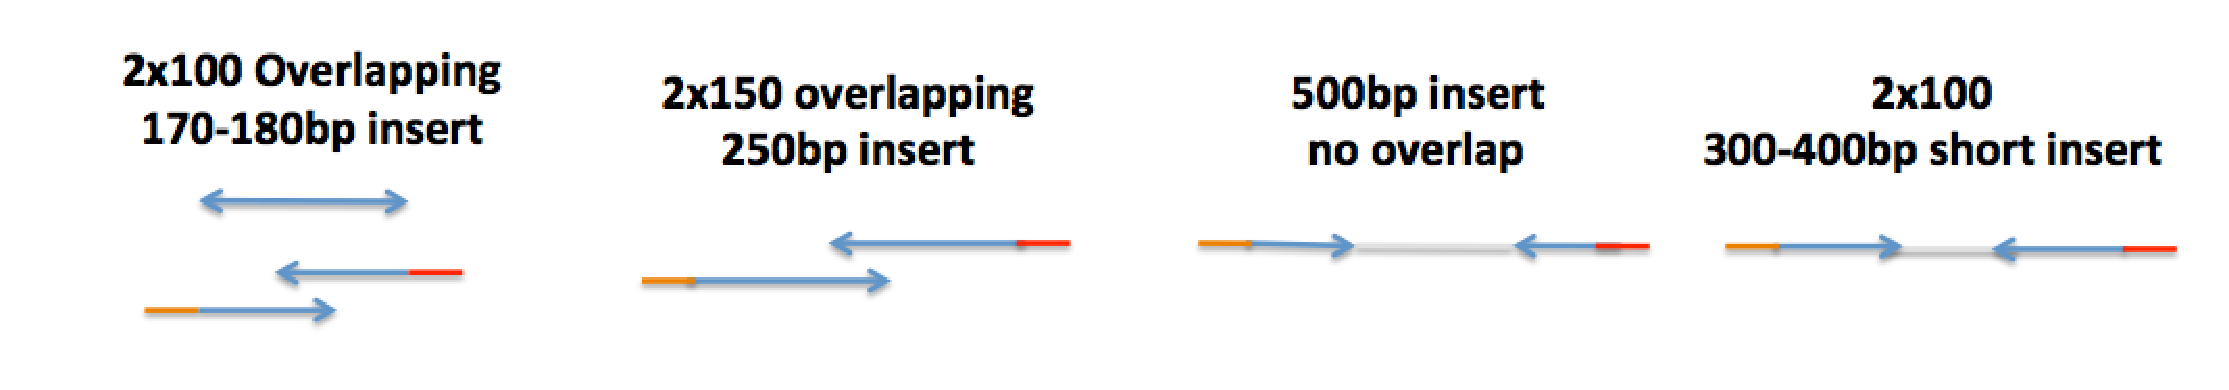
\includegraphics[scale=.35]{imgs/image1.eps}
%
% If the width of the figure is less than 7.8 cm use the \texttt{sidecapion} command to flush the caption on the left side of the page. If the figure is positioned at the top of the page, align the sidecaption with the top of the figure -- to achieve this you simply need to use the optional argument \texttt{[t]} with the \texttt{sidecaption} command}
\label{fig:1}       % Give a unique label
\end{figure}

\begin{figure}
%\sidecaption[t]
\caption{Examples of complete libraries. Figure2a shows an example of a TruSeq library with a narrow range peaking around 1kb. Figure 2b shows an example of a TruSeq library with a narrow range peaking around 360~bp. Figure 2c shows an example of a TruSeq library with a narrow range peaking around 700~bp. Figure 2d shows an example of a TruSeq library with a broad range peaking around 450. Figure 2e shows an example of a Nextera library peaking around 1,600~bp.  }
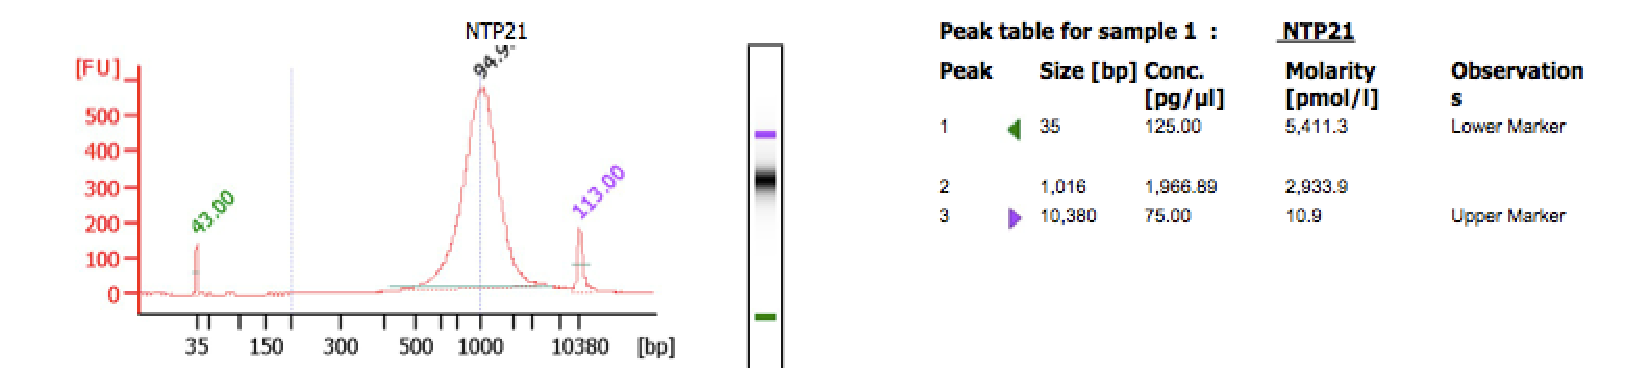
\includegraphics[width=12cm]{imgs/image2.eps}
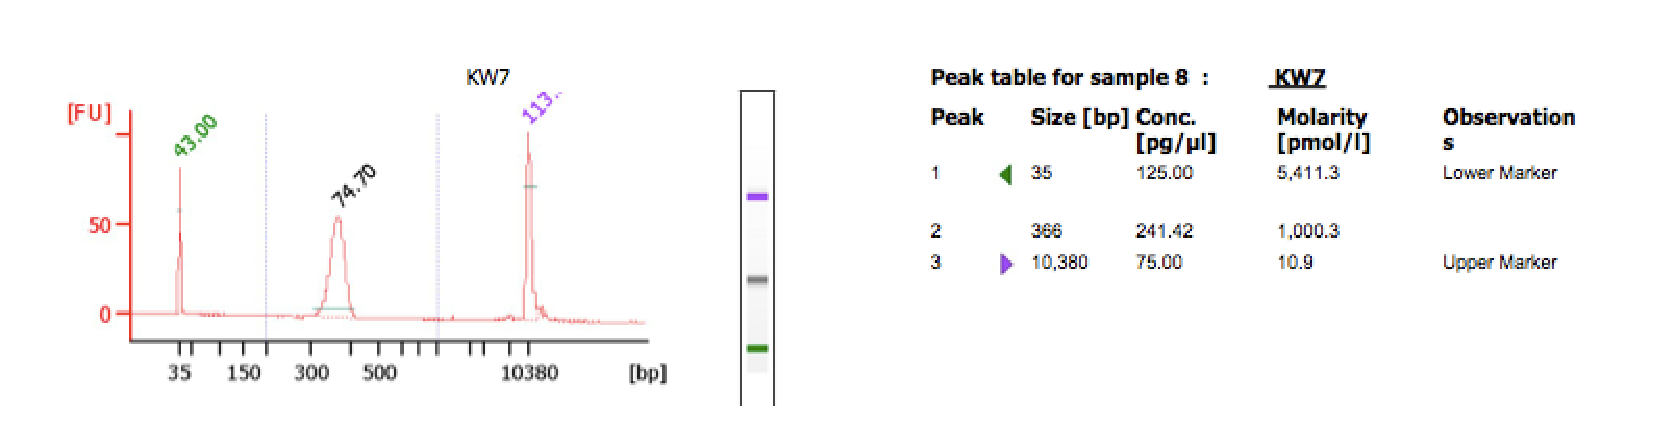
\includegraphics[width=12cm]{imgs/image3.eps}
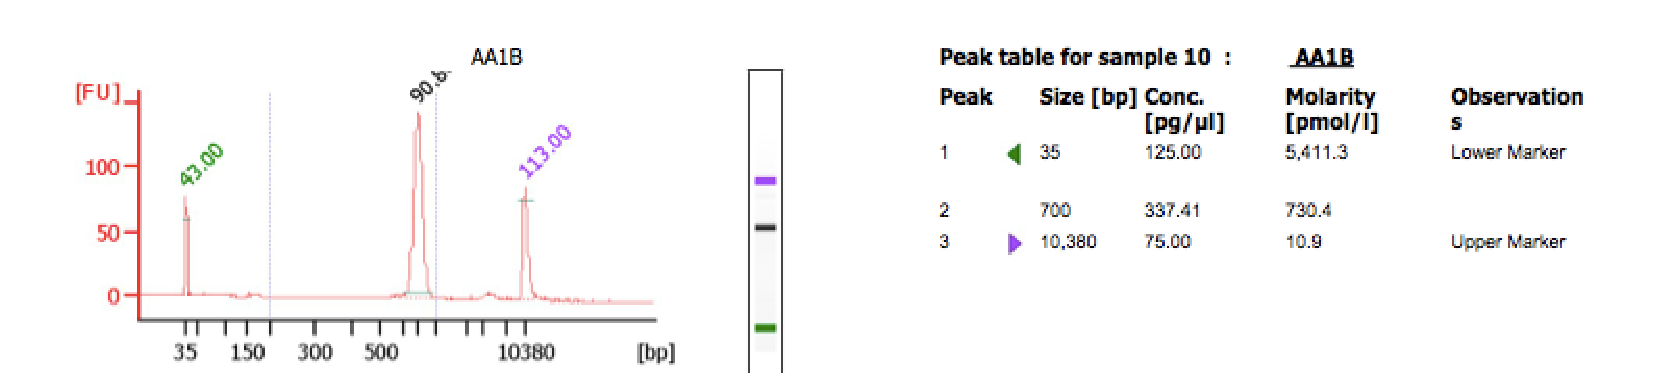
\includegraphics[width=12cm]{imgs/image4.eps}
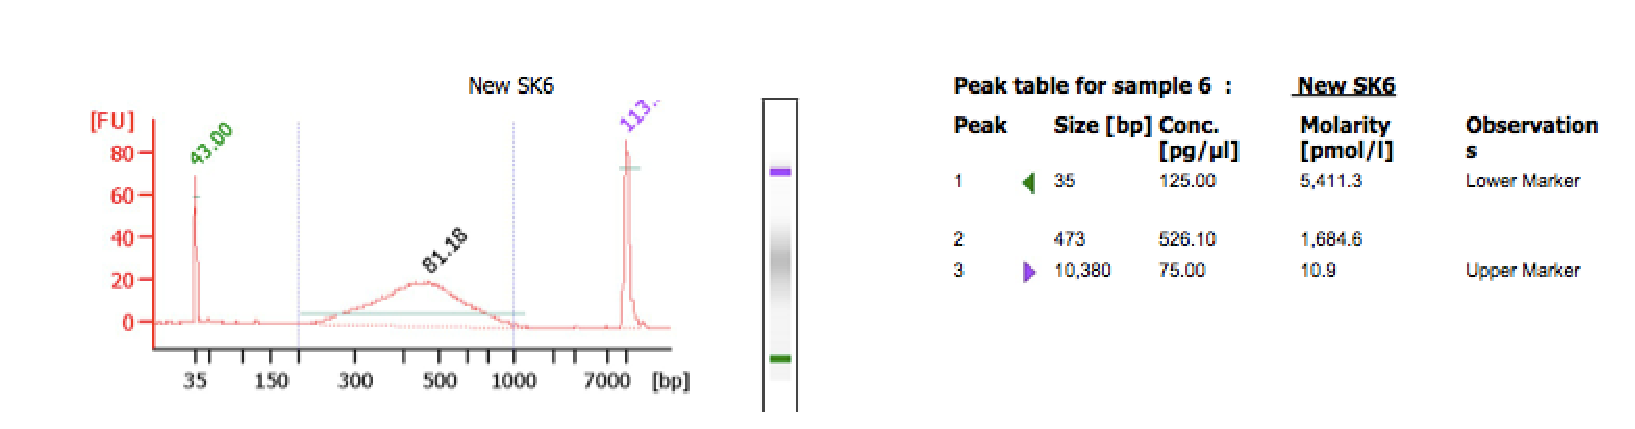
\includegraphics[width=12cm]{imgs/image5.eps}
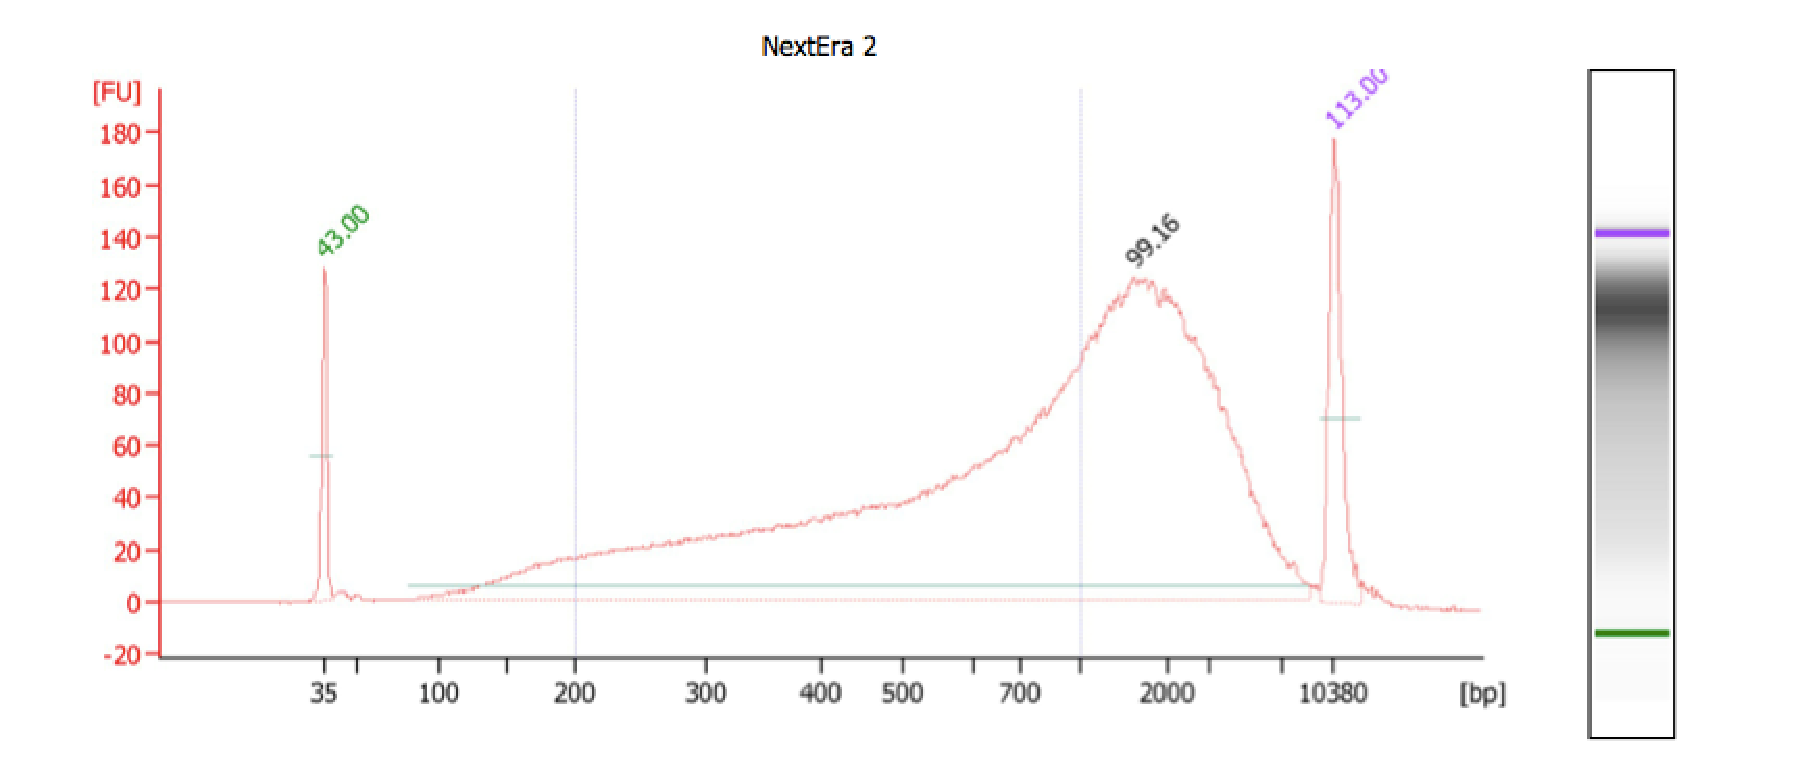
\includegraphics[width=6cm]{imgs/image6.eps}
%
%\caption{Please write your figure caption here}
\caption{ }
% If the width of the figure is less than 7.8 cm use the \texttt{sidecapion} command to flush the caption on the left side of the page. If the figure is positioned at the top of the page, align the sidecaption with the top of the figure -- to achieve this you simply need to use the optional argument \texttt{[t]} with the \texttt{sidecaption} command}
\label{fig:2}       % Give a unique label
\end{figure}

% Use the \index{} command to code your index words

%
\begin{acknowledgement}
If you want to include acknowledgments of assistance and the like at the end of an individual chapter please use the \verb|acknowledgement| environment -- it will automatically render Springer's preferred layout.
\end{acknowledgement}
%

%%%%%%%%%%%%%%%%%%%%%%%% referenc.tex %%%%%%%%%%%%%%%%%%%%%%%%%%%%%%
% sample references
% %
% Use this file as a template for your own input.
%
%%%%%%%%%%%%%%%%%%%%%%%% Springer-Verlag %%%%%%%%%%%%%%%%%%%%%%%%%%
%
% BibTeX users please use
% \bibliographystyle{}
% \bibliography{}
%

\begin{thebibliography}{99.}%
% and use \bibitem to create references.
%
%
% Use the following syntax and markup for your references if 
% the subject of your book is from the field 
% "Computer Science, Economics, Engineering, Geosciences, Life Sciences"
%
%
\bibitem{Brown} Brown B, Aaron M (2001) The politics of nature. In: Smith J (ed) The rise of modern genomics, 3rd edn. Wiley, New York 

\bibitem{MG-RAST}F Meyer, D Paarmann, M D'Souza, R Olson, EM Glass, M Kubal, T Paczian, A Rodriguez, R Stevens, A Wilke, J Wilkening, RA Edwards (2008). The metagenomics RAST server – a public resource for the automatic phylogenetic and functional analysis of metagenomes. BMC Bioinofmatics. 9:386. doi:10.1186/1471-2105-9-386

\bibitem{Mason-deepwater} Mason, O., Hazen T., Borglin, S., Chain, P., Dubinsky, E., Fortney, J., et al. (2012). Metagenome, metatranscriptome and single-cell sequencing reveal microbial response to Deepwater Horizon oil spill. The ISME journal, 6(9), 1715-1727

\bibitem{Korenblum} Korenblum E., Souza DB., Penna M, Seldin L. (2013). Molecular Analysis of the Bacterial Communities in Crude Oil Samples from Two Brazilian Offshore Petroleum Platforms. International Journal of Microbiology Volume 2012. doi:10.1155/2012/156537
Lorenz P and Eck J. (2005). Metagenomics Industrial Applications. Nature Reviews Microbiology 3, 510-516. doi:10.1038/nrmicro1161

\bibitem{Hampton-Marcell} Hampton-Marcell JT., Moormann SM., Owens SM., Gilbert JA. (2013) Preparation and Metatranscriptomic Analyses of Host-Microbe Systems in Microbial Metatgenomics, Metatranscrtomics, and Metaproteomics volume 531 issue 169. Academic Press. ISBN 978-0-12-407863-5. ISSN 0076-6879.

\bibitem{Rubin} Rubin BER., Gibbons SM., Kennedy S., Hampton-Marcell J., Owens S., Gilbert J. (2013) Investigating the Impact of Storage Conditions on Microbial Community Composition in Soil Samples. PLOSone. DOI: 10.1371/journal.pone.0070460

\bibitem{Segata} Segata, N., Boernigen D., Tickle TL., Morgan XC., Garrett WS, Huttenhower C. (2013) Computational Meta’omics for Microbial Community Studies. Molecular Systems Biology, doi: 10.1038/msb.2013.22

\bibitem{MIE} Thomas, T., Gilbert, J., Meyer, F. (2012). Metagenomics – a guide from sampling to data analysis. Microbial Informatics and Experimentation, 2, doi:10.1186/2042-5783-2-3

\bibitem{Wang}Wang LY., Ke WJ., Sun XB., Liu JF., Gu JD., Mu BZ. (2013). Comparison of bacterial community in aqueous and oil phases of water-flooded petroleum reservoirs using pyrosequencing and clone library approaches. Appl Microbiol Biotechnol. DOI 10.1007/s00253-013-5472-y

\bibitem{API} A Wilke, J Bischof, T Harrison, T Brettin, M D'Souza, W Gerlach, HMatthews, T Paczian, J Wilkening, E M Glass, N Desai, F Meyer. (2015) A RESTful API for Accessing Microbial Community Data for MG-RAST. PLOS: Computational Biology. DOI: 10.1371/journal.pcbi.1004008
%
% Online Document
%\bibitem{basic-online} Dod J (1999) Effective Substances. In: The dictionary of substances and their effects. Royal Society of Chemistry. Available via DIALOG. \\
%\url{http://www.rsc.org/dose/title of subordinate document. Cited 15 Jan 1999}
%
% Journal article by DOI
%\bibitem{basic-DOI} Slifka MK, Whitton JL (2000) Clinical implications of dysregulated cytokine production. J Mol Med, doi: 10.1007/s001090000086
%
% Journal article
%\bibitem{basic-journal} Smith J, Jones M Jr, Houghton L et al (1999) Future of health insurance. N Engl J Med 965:325--329
%
% Monograph
%\bibitem{basic-mono} South J, Blass B (2001) The future of modern genomics. Blackwell, London 
%
\end{thebibliography}

\end{document}
